\mainmatter

\section{Introduction}\label{introduction}

{[}Revision 3 changelog{]}

\begin{itemize}
\itemsep1pt\parskip0pt\parsep0pt
\item
  grounded the problem with numbers on disasters
\item
  re-grouped results in to research paper, contributions and
  exploitations
\item
  added a table with the list of invention registered at TTO
\item
  added a brief explanation of each contribution
\item
  results section is renamed ``research outcomes''
\item
  improved the research questions
\item
  added figures
\end{itemize}

\subsection{Problem Statement}\label{problem-statement}

\reversemarginpar

This thesis is about how to improve crisis training with ICT
technologies. Crisis training is an umbrella term for complex,
collaborative activities aiming at improving people's ability for
\emph{preparedness} to human and natural-caused disasters (e.g.~a
flooding or a terrorist attack) {[}@Lagadec:1997js{]}. Disasters have a
huge impact on societies, both in terms of human lives and costs: over
the last 35 years, the frequency of disasters have increased five-fold;
the damage caused has multiplied by approximately eight times\footnote{Source:
  ``Council adopts new Union Civil Protection Mechanism'' Available at:
  www.consilium.europa.eu/uedocs/cmsdata/docs/pressdata/en/jha/140108.pdf.}.
According with the UN Office for Disaster Risk reduction, over the
decade 1992-2012, disasters have affected 4.4 billion people and have
caused 2 trillion USD in damages worldwide\footnote{Source: The United
  Nation Office for Disaster Risk Reduction (http://unisdr.org)}. For
this reason training for better crisis management, hereafter
\emph{crisis training} is a priority for many countries, including the
European ones.

Beside teaching the population what to do when a disaster occurs, crisis
training focuses on teaching workers (e.g.~firefighters, paramedics) how
to efficiently respond to a crisis; for example by actuating coping
strategies and implementing rescue procedures (crisis management). Each
crisis is likely to be a specific, unpredictable event that will not
take place again under the same circumstances. Training for crisis
preparedness is a wicked problem, however better crisis management can
positively affect everyone's lives.

There are four main approaches to crisis training: protocol training,
tabletop exercises, physical simulations and serious games; on top of
that real crises also offer triggers for learning
{[}@Deverell:2009fk{]}. In this research work we look at medium to large
scale physical simulations and serious games as key training
practices.\todo{box with example simulation?} Physical simulations
recreate at best real crises in terms of environment (e.g.~presence of
debris, collapsed buildings), and in reproducing feelings experienced by
crisis worker such as stress, tension, time pressure and uncertainty
{[}@Borodzicz:2002em{]}. Yet these events are arranged rarely. This due
to the high set-up cost and the large effort required to coordinate
multiple organisations and dozens of field workers. Moreover it has been
observed that the impact of those events is limited by lack of
technologies, for example for capturing data to maintain an overview of
rescue efforts {[}@Kyng:2006he{]} and to support post-simulation
debriefing {[}@Mora:2012vc{]}. On the other end, serious games trade the
realism of physical simulations to provide a more lightweight training
experience which can be reproduced frequently by single workers or
teams; adding the ``fun'' element as motivator to engage workers in
frequent play {[}@DiLoreto:2012jj{]}. The two approaches are not
mutually exclusive but rather complementary.
\todo{focus only on physical sim. not talking about serious games for now?}

\begin{quote}
\emph{Hence, how is it possible to maximise crisis training learning
outcomes during physical or game-based simulation of crisis work}?
\end{quote}

\begin{quote}
\emph{The training practices already in place can be enhanced by
combining (i) reflective, experience-based learning practices and (ii)
advances in ICT and sensing-based interaction}.
\end{quote}

Experience-based learning is a powerful tool. Facilitating learning from
work experiences of the different roles on field (e.g.~disaster managers
vs.~field workers) can bring outcomes to complement traditional formal
training. Learning from experiences entails reflection
{[}@boud1985reflection; @Dewey:1998ug; @kolb1974toward{]}. Reflection on
action has been a research topic since the work of Dewey
{[}@dewey1933we{]} that describes how we learn by comparing our
expectations to new and past experiences in order to promote continuous
learning. Reflecting on action is critical in order to learn from past
experiences with the goal of performing better in the future
{[}@boud1985reflection; @Schon:1983ut{]}; and a number of tools have
been developed to support reflection, as an individual or collaborative
activity. Among those, the CSRL (Computer Supported Reflective Learning)
model developed as part of the MIRROR project\footnote{MIRROR Project -
  http://www.mirror-project.eu} aims at providing guidelines to develop
technology tools to support reflection. It identifies a cycle of four
stages of reflection {[}@Krogstie:2013kf{]}: \emph{do work},
\emph{initiate reflection session}, \emph{conduct reflection session}
and \emph{apply reflection outcomes}. For each stage a number of
reflection-useful activities that can be augmented with technology are
provided. In the context of crisis training, three activities are
addressed: (i) capturing work experiences (ii) re-creating work
experiences (iii) generating new work experiences. Technology provides
help in different ways. Sensors can capture aspects of work experiences;
data which can be visualised on a interactive computer interface to
provide triggers for re-evaluating an experience towards a learning
outcome, or that can be used to plan new training work.

Yet current technology tools don't consider the very particular,
situated nature of crisis work. While data capturing tools lack of
interaction paradigms suitable to be used in-action, visualisation tools
struggle in providing the users with context information needed to
ground the reflection process towards a learning outcome.

Theories in the field of \emph{sensing-based interaction}
{[}@Zhai:2005jm{]}, can inform the design of technologies to better
assist reflective crisis training. Sensing-based interaction is a trend
in HCI make interaction with ICT systems intuitive and effective.
\emph{Tangible} and \emph{embodied} {[}@Dourish:2001vc{]} are two
characterising traits of such interfaces. They aim at enabling
interaction with digital information exploiting the affordances that
everyday objects provide, rather than traditional input devices such as
keyboard, mouse or touchscreens. Using sensor-based technology,
conventional object can be augmented and turned in ``physical handles''
to digital operations {[}@Ishii:1997ur{]}, linking their traditional
affordances to new digital meanings.\todo{improve this paragraph…} Yet
building prototypes of sensing-based interfaces, is a complex task
requiring both software and hardware engineering skills. Moreover
prototypes to support crisis training during physical simulation need to
be employed in harsh environments requiring high resilience.

\begin{figure}[tbh]
    \centering
    \includegraphics[width=0.70\textwidth]{better_management}
    \caption{Relation among the three domain of this thesis}
    \label{fig:topic_relation}
\end{figure}

Embodied interaction techniques can be implemented in computer
interfaces to allow \emph{capturing work experiences} disrupting as
little as possible the rescue work, to \emph{re-create work experiences}
in a physical context for debriefing purposes and to \emph{generate new
work experiences} for continuous training characterised by engaging,
playful interaction and reduced cost compared to traditional physical
simulations.\todo{This is the research result, need to add research contributions as well?}

\subsection{Research methodology}\label{research-methodology}

The work in this thesis is based on design research {[}@Hevner:2010fy;
@March:1995gm{]}. The work followed a \emph{user centred approach}
{[}@MAGUIRE:2001dp; @Gulliksen:2003hd{]}, based on exploratory studies
and design work following in multiple iterations.

Several qualitative research methods {[}@robson1993real{]} have been
adopted, including shadowing of workers, observations and interviews
during field studies. Scenarios, personas and mockups aided the
user-centred design work. These activities were functional to the
\emph{design research} approach. Consistently with this methodology,
grounded on the activities of \emph{building} artefacts for a specific
purpose and of \emph{evaluating} how well the artefacts perform
{[}@March:1995gm{]}, a number of prototyping iterations and evaluation
studies have been performed.

Prototyping involved the construction of hardware and software systems
to support reflection processes. The design of prototypes was grounded
in field studies during physical simulations of crisis I attended.
Simple prototypes were initially used to build a deeper understanding of
the crisis domain, for which I didn't have a previous knowledge. They
acted as technology probes {[}@Hutchinson:2003il{]} and facilitate
building and understanding of the crisis domain by engaging users in
focus groups. Later, multiple iterations implemented a growing set of
requirements in fully working prototypes robust enough to be deployed
during simulated rescue work.

User evaluations followed each design iteration. The aim was both in
assessing usability of the prototypes and relevance of reflection
outcomes they might produce. Prototypes were evaluated both during focus
groups and during large simulations of crisis response works. Results
from evaluations have fed following design iterations, contributed in
the validation of theory models on reflective learning and into the
development of new conceptual works.

\begin{figure}[tbh]
    \centering
    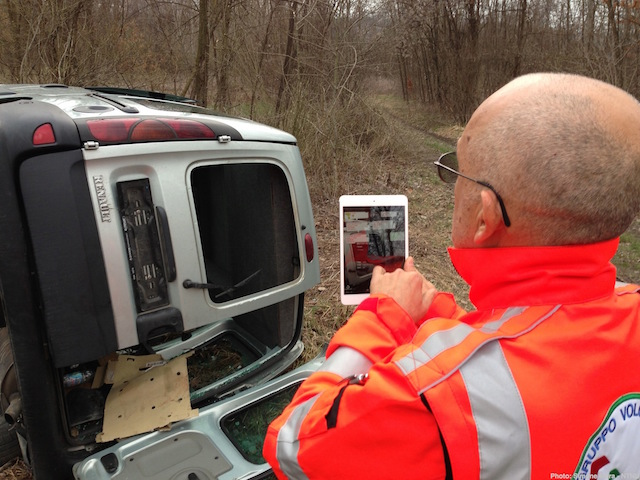
\includegraphics[width=1\textwidth]{introduction_cromar}
    \caption{One of the evaluation studies performed}
    \label{fig:cromar}
\end{figure}

\subsection{Research questions}\label{research-questions}

The main research question for the PhD work is:

\begin{quote}
MRQ: What are the opportunities to promote reflection in crisis training
with sensing-based interfaces?
\end{quote}

To answer the main research question the work has been broken down into
three sub-questions:

\begin{quote}
RQ1: How sensing-based interfaces can be designed to enable unobtrusive
data collection during crisis work?
\todo{should refocus RQ1 with more attention to understanding the domain?}
\end{quote}

\begin{quote}
RQ2: How sensing-based interfaces can be designed to trigger and support
reflection activities?
\end{quote}

\begin{quote}
RQ3: How sensing-based technologies for supporting reflection can be
rapid prototyped?
\end{quote}

While the first two questions aim at investigating the design of systems
to support with technology the tasks of capturing, re-creating and
generating work experiences; the third question investigates how
toolkits and open-source communities can ease the implementation of
design ideas into prototypes.

\subsection{Research outcomes}\label{research-outcomes}

Three are the main outcomes of this PhD work. Research papers in
peer-reviewed conferences and journal answered the research questions. A
body of knowledge in the field of technology enhanced learning

\subsubsection{Research papers}\label{research-papers}

The research questions RQ1-RQ3 are addressed in the following research
papers:

\begin{quote}
\textbf{P1} Mora, S., Boron, A., \& Divitini, M. (2012). CroMAR: Mobile
Augmented Reality for Supporting Reflection on Crowd Management.
\emph{International Journal of Mobile Human Computer Interaction}, 4(2),
88--101.
\end{quote}

\begin{quote}
\textbf{P2} Mora, S., \& Divitini, M. (2014). Supporting Debriefing with
Sensor Data: A Reflective Approach to Crisis Training. \emph{In
Proceeding of Information Systems for Crisis Response and Management in
Mediterranean Countries, ISCRAM-MED}, 196(Chapter 7), 71--84.
\end{quote}

\begin{quote}
\textbf{P3} Mora, S., \& Divitini, M. (2014). WATCHiT: a modular and
wearable tool for data collection in crisis management and training.
\emph{In Proceeding of the European Conference in Ambient Intelligence,
AMI}.
\end{quote}

\begin{quote}
\textbf{P4} Di Loreto, I., Mora, S., \& Divitini, M. (2012). Don't
Panic: Enhancing Soft Skills for Civil Protection Workers. \emph{In
Proceeding of International Conference on Serious Games Development
Applications, SGDA}, 7528(Chapter 1), 1--12.
\end{quote}

\begin{quote}
\textbf{P5} Mora, S., Di Loreto, I., \& Divitini, M. A token-constraint
approach to interactive board games: the case of ``Don't Panic!''.
\emph{To Be Submitted at INTERACT2015}.
\end{quote}

\begin{quote}
\textbf{P6} Müller, L., Divitini, M., Mora, S., Rivera-Pelayo, V., \&
Stork, W. Context Becomes Content: Sensor Data for Computer Supported
Reflective Learning. \emph{To Appear in the IEEE Transactions on
Learning Technologies}.
\end{quote}

\begin{quote}
\textbf{P7} Mora, S., \& Farshchian, B. A. (2010). A Unified
Architecture for Supporting Direct Tag-Based and Indirect Network-Based
Resource Discovery. \emph{In Proceeding of the International Conference
on Ambient Intelligence, AMI}, 6439(Chapter 20), 197--206.
\end{quote}

Table x shows the mapping between research papers and research
questions.

\begin{longtable}[c]{@{}lccccccc@{}}
\caption{Mapping between research papers and research
questions}\tabularnewline
\toprule
\begin{minipage}[b]{0.37\columnwidth}\raggedright\strut
Research questions
\strut\end{minipage} &
\begin{minipage}[b]{0.05\columnwidth}\centering\strut
P1
\strut\end{minipage} &
\begin{minipage}[b]{0.05\columnwidth}\centering\strut
P2
\strut\end{minipage} &
\begin{minipage}[b]{0.05\columnwidth}\centering\strut
P3
\strut\end{minipage} &
\begin{minipage}[b]{0.05\columnwidth}\centering\strut
P4
\strut\end{minipage} &
\begin{minipage}[b]{0.05\columnwidth}\centering\strut
P5
\strut\end{minipage} &
\begin{minipage}[b]{0.05\columnwidth}\centering\strut
P6
\strut\end{minipage} &
\begin{minipage}[b]{0.05\columnwidth}\centering\strut
P7
\strut\end{minipage}\tabularnewline
\midrule
\endfirsthead
\toprule
\begin{minipage}[b]{0.37\columnwidth}\raggedright\strut
Research questions
\strut\end{minipage} &
\begin{minipage}[b]{0.05\columnwidth}\centering\strut
P1
\strut\end{minipage} &
\begin{minipage}[b]{0.05\columnwidth}\centering\strut
P2
\strut\end{minipage} &
\begin{minipage}[b]{0.05\columnwidth}\centering\strut
P3
\strut\end{minipage} &
\begin{minipage}[b]{0.05\columnwidth}\centering\strut
P4
\strut\end{minipage} &
\begin{minipage}[b]{0.05\columnwidth}\centering\strut
P5
\strut\end{minipage} &
\begin{minipage}[b]{0.05\columnwidth}\centering\strut
P6
\strut\end{minipage} &
\begin{minipage}[b]{0.05\columnwidth}\centering\strut
P7
\strut\end{minipage}\tabularnewline
\midrule
\endhead
\begin{minipage}[t]{0.37\columnwidth}\raggedright\strut
(1) How computer interfaces can be designed to enable unobtrusive data
collection during crisis work?
\strut\end{minipage} &
\begin{minipage}[t]{0.05\columnwidth}\centering\strut
\strut\end{minipage} &
\begin{minipage}[t]{0.05\columnwidth}\centering\strut
*
\strut\end{minipage} &
\begin{minipage}[t]{0.05\columnwidth}\centering\strut
*
\strut\end{minipage} &
\begin{minipage}[t]{0.05\columnwidth}\centering\strut
\strut\end{minipage} &
\begin{minipage}[t]{0.05\columnwidth}\centering\strut
\strut\end{minipage} &
\begin{minipage}[t]{0.05\columnwidth}\centering\strut
*
\strut\end{minipage} &
\begin{minipage}[t]{0.05\columnwidth}\centering\strut
\strut\end{minipage}\tabularnewline
\begin{minipage}[t]{0.37\columnwidth}\raggedright\strut
(2) How interaction techniques can be designed to facilitate the
different phases of a reflection processes?
\strut\end{minipage} &
\begin{minipage}[t]{0.05\columnwidth}\centering\strut
*
\strut\end{minipage} &
\begin{minipage}[t]{0.05\columnwidth}\centering\strut
*
\strut\end{minipage} &
\begin{minipage}[t]{0.05\columnwidth}\centering\strut
\strut\end{minipage} &
\begin{minipage}[t]{0.05\columnwidth}\centering\strut
*
\strut\end{minipage} &
\begin{minipage}[t]{0.05\columnwidth}\centering\strut
*
\strut\end{minipage} &
\begin{minipage}[t]{0.05\columnwidth}\centering\strut
*
\strut\end{minipage} &
\begin{minipage}[t]{0.05\columnwidth}\centering\strut
\strut\end{minipage}\tabularnewline
\begin{minipage}[t]{0.37\columnwidth}\raggedright\strut
(3) How technology tools for supporting reflection can be rapid
prototyped?
\strut\end{minipage} &
\begin{minipage}[t]{0.05\columnwidth}\centering\strut
\strut\end{minipage} &
\begin{minipage}[t]{0.05\columnwidth}\centering\strut
\strut\end{minipage} &
\begin{minipage}[t]{0.05\columnwidth}\centering\strut
*
\strut\end{minipage} &
\begin{minipage}[t]{0.05\columnwidth}\centering\strut
\strut\end{minipage} &
\begin{minipage}[t]{0.05\columnwidth}\centering\strut
*
\strut\end{minipage} &
\begin{minipage}[t]{0.05\columnwidth}\centering\strut
\strut\end{minipage} &
\begin{minipage}[t]{0.05\columnwidth}\centering\strut
*
\strut\end{minipage}\tabularnewline
\bottomrule
\end{longtable}

Results were exploited in two directions. On one end they forged the
research contributions of this PhD work. On the other end the drove an
investigation of commercial relevance for the technologies developed.

\subsubsection{Research contributions}\label{research-contributions}

The seven paper published added to the following contributions of this
research work.

\begin{quote}
\emph{\textbf{C1:} Implementation and evaluation of MIRROR Computer
Supported Reflective Learning theory.} It includes a validation of
previous theoretical models available in literature and in the
formulation of new theories
\end{quote}

\begin{quote}
\emph{\textbf{C2:} Knowledge about designing data capturing tools for
crisis workers.} It provides a definition of the design paces as well as
design challenges for helping designers and engineers in building
computer-based data capturing tools.
\end{quote}

\begin{quote}
\emph{\textbf{C3:} Novel sensing-based interaction techniques to support
re-creation and generation of work experiences in crisis training} It
describes novel user interfaces for the visualisation and manipulation
of data captured from working experiences.
\end{quote}

\begin{quote}
\emph{\textbf{C4:} Knowledge about implementing prototypes to be
deployed into the wild.} It presents information about software and
hardware tools, techniques and frameworks to ease the manufacture of
sensing-based interfaces prototypes.
\end{quote}

\begin{figure}[htbp]
\centering
\includegraphics{imgs/papers-contributions-mapping.pdf}
\caption{Relation between papers and contributions}
\end{figure}

\begin{figure}[tbh]
    \centering
    \includegraphics{papers-contributions-mapping}
    \caption{Relation between papers and contributions}
    \label{fig:mapping}
\end{figure}

These contributions are relevant for several research communities
including Technology Enhanced Learning (C1), Tangible Embodied Embedded
Computing (C3, C4), Information systems for Crisis Response (C1,C2)

\subsubsection{Exploitation of research
results}\label{exploitation-of-research-results}

During the final phase of the investigation, commercial exploitation of
research results has been investigated. The focus was in assessing
efforts needed and path of actions to evolve the prototypes developed as
theory demonstrator into commercial products. To this end, I co-authored
five \emph{Disclosure of invention} (DOFI): technical documents that
capture the description of the technologies created and establish
inventor-ship. DOFIs were drafted based on information published in
research paper (Table X)

\begin{table}[h]
\begin{tabular}{p{\dimexpr 0.30\linewidth-2\tabcolsep}p{\dimexpr 0.50\linewidth-2\tabcolsep}p{\dimexpr 0.20\linewidth-2\tabcolsep}}
\toprule
Inventors                              & Invention  & Relation to Research papers  \\ \midrule
Mora, S., Boron, A. and Divitini, M.   & CroMAR. Situated reflection and training in crisis management.   & P1, P2    \\
Mora, A. and Divitini, M. & WATCHiT. Wearable data collection in crisis management and training & P2, P3 \\
Di Loreto, I., Mora, S. and Divitini, M. & “Don’t Panic!” A serious game for enhancing soft skills for Civil Protection workers & P4, P5 \\
Mora, S., Di Loreto, I. and Divitini, N. & Anyboard: a platform for creating and play digital board games & P5 \\
Mora, S. and Divitini, M. & TILES Toolkit. Building seamless interfaces between people and the Internet of Things & P3, P5 \\
\bottomrule
\end{tabular}
\caption{My caption}
\label{my-label}
\end{table}

Disclosure of inventions were registered at NTNU Technology Transfer
office, a business facilitator affiliated with NTNU, in accordance with
the Norwegian law\footnote{In accordance with
  ``Arbeidstakeroppfinnelsesloven'', ``Universitets og høgskoleloven''
  and NTNU's internal Guidelines for innovation}. They were used by
technology transfer managers to assess patent applicability and
establishment of commercial activities. To this effort, I presented
research results to several subjects from the industries working in the
emergency management field, raising positive and supportive feedbacks.
\sout{I further refined rapid prototyped ideas during an Hackaton at MIT
Media Lab} In November 2014 I was granted by NTNU Discovery \footnote{NTNU
  Discovery - http://ntnudiscovery.no} a 150.000NOK
(\textasciitilde{}22.000USD) seed for financing further commercial
exploration of the research results after the completion of my PhD.

\subsection{Context of the work}\label{context-of-the-work}

This research work is framed within the EU-funded (IST-FP7) project
MIRROR. The focus of MIRROR is the creation of a set of technology
applications that enable employees to learn from their own and others'
experiences to perform better in the future. As an associate researcher
of MIRROR I took part in shaping the results of the projects by
designing and implementing ICT systems, writing deliverables and
attending project meetings. Thanks to MIRROR I cooperated with crisis
workers associations partner of the consortium to run user and
evaluation studies. I also benefited from discussions and joined works
and publications with the members of the consortium. After the scheduled
final review in September 2014, MIRROR has been graded as ``Excellent''
by the EU commission.

During the PhD I worked as visiting researcher in two foreign
institutions: City London University\footnote{City London University -
  http://city.ac.uk} and MIT SENSEable City Lab\footnote{MIT SENSEable
  City Laboratory - http://senseable.mit.edu}. The purpose of the two
visits was to investigate whether the technologies developed during the
PhD could be generalised to application domains that share similarities
with crisis training.

During fourteen weeks spent at City University (partner of the MIRROR
consortium) I investigated the design and production of a digitally
augmented serious game for better training of dementia carers, under the
supervision of professor Neil Maiden. The game has been implemented and
evaluated in eight care homes in the greater London area, and is
reported in a joined publication to be submitted.

During twelve weeks spent at the MIT SENSEable City Lab I investigated
the design and production of a tangible interface to promote user
engagement and reflection about urban-mobility data under the
supervision of professor Carlo Ratti. The work has been has been
displayed to the public in two exhibitions: ``Wave'' currently held in
Paris and ``CNR Internet Festival'' held in Pisa, Italy.

I also co-advised thesis works of eight master student who have
contributed in the development of prototypes. One of them also
co-authored P1.

\subsection{Structure of the thesis}\label{structure-of-the-thesis}

The thesis is structured as follows:

\textbf{Chapter 2} introduces the Crisis domain providing an overview on
scenarios, activities and roles; and presenting debriefing as a tool for
experiential learning.

\textbf{Chapter 3} describes relevant background theory on reflective
and experience-based learning with focus on describing the Computer
Supported Reflective Learning model adopted as theoretical underpinning
of this research work.

\textbf{Chapter 4} presents relevant background theory in sensing
based-interaction, motivating the use of that category of applied to
reflective learning.

\textbf{Chapter 5} depicts the research strategy and approach adopted by
this PhD work, giving and overview of the user studies conducted and
prototypes built.

\textbf{Chapter 6} summarises the results for the research papers.

\textbf{Chapter 7} outlines the contribution of this thesis and their
relations to the research papers.

\textbf{Chapter 8} proposes an evaluation of the work done.

\textbf{Chapter 9} concludes the thesis and sketches out future research
and innovation works.

\textbf{Appendix A} contains the research papers P1-P7.

\textbf{Appendix B} contains research papers that were written during
the research fellowship but that were outside the main scope of the
work.\todo{Do we want to add this?}

\textbf{Appendix C} includes a benchmark of hardware toolkits for rapid
prototyping which has been used to select the specific tools used to
implement the prototypes in this PhD.
